\documentclass{article}
\usepackage{times}
\usepackage{graphicx}
\usepackage{subfigure} 
\usepackage{hyperref}
\usepackage{amsmath}
\usepackage{amssymb}
\usepackage{color}
\begin{document}
	%Ghassen
	\section{LM ARIMA}
		\subsection{Exploratory Analysis}
		We used the Autocorrelation Function to explore possible AR or MA terms. Reminder: AR is for the AutoRegressive terms = autocorrelated lags and MA is for the Mean Average terms (non-linear model and the underlying implementation uses Kalman filters).
	
		\subsection{Training/Testing Strategy}
	We resorted to walk forward optimization (moving window training) which is a form of k-fold cross-validation for time series data. We have a moving window of the time series and at each instance of the window we re-estimate the coefficients and do look-ahead predictions. This helps to average out the error measures as well as devise an online strategy for trading.
	However, it would be expensive to re-estimate the order (number of lags or MA terms) at each step. Therefore, we use auto.arima() one time to explore the order inferred by all of the testing data then refit to that order in each window: re-estimate the AR and MA coefficients but fix the order. 
	The criterion for our training would be AIC (a lower AIC indicates a higher log-likelihood thus a high predictable power while penalizing for number of terms: regularization) for ARIMA. As for the linear model, it could be AIC as well (computation is off by a constant in R for AIC in LM and ARIMA so it is hard to compare) but we focused on the p-value of each regressor and the general R-squared for the training fit and the visual analysis of the results as well as the Mean Absolute Error (or Mean Scaled Error).
	
\begin{center}	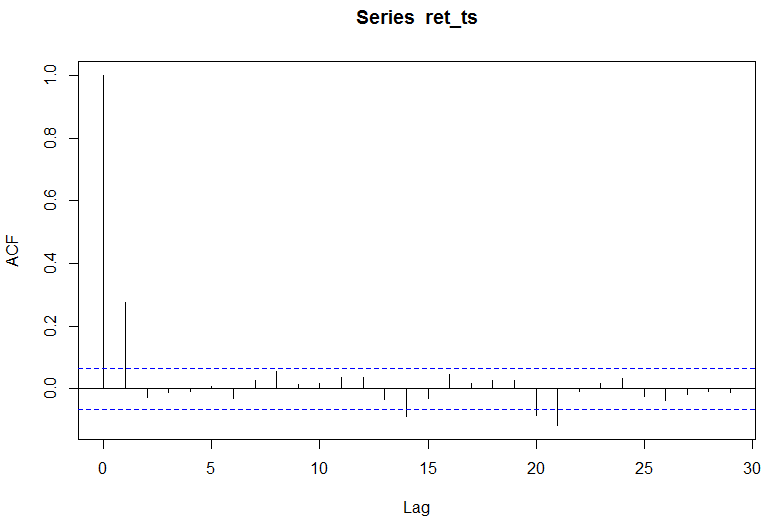
\includegraphics[scale=0.7]{../ACF.PNG}\end{center}
	\subsection{ARIMA}
	As seen in the ACF plot, there are 5 autocorrelated lags wihin a close range. However, auto.arima struggles with the scale of our data to explore more than 2 MA terms and 3 AR terms so it picks a model of AR(3)MA(1) or AR(2)MA(2). The MA terms lead to a non-linear system, therefore, our later LM analysis is not expressing the whole data.
	
	Using ARIMA, we faced lots of issues with the convergence given singularity problems in the design matrix. This amounted to 2 distinct problems: multicollinearity: was easy to remove linearly dependent columns using QR decomposition but high correlation between the columns was hard to analyse AND the number of variables exceeding the number of observations. Therefore, we used Variance Inflation Factors to analyze the correlation between columns and eliminate those that exceeded a certain threshold. Afterwards, we had to reduce our dimensions to be able to fit smaller windows of the time series: we used PCA where we found that 95$\%$ of the variance was contributed by the first 200 of the 808 columns and thus used those for ARIMA.
	
	However, ARIMA still takes too long. auto.arima() on the hold dataset is more than 7 hours (before PCA). The values after PCA had a worse AIC (a criterion of fitness) and we still have to decide on the best window size.
	\begin{center}
	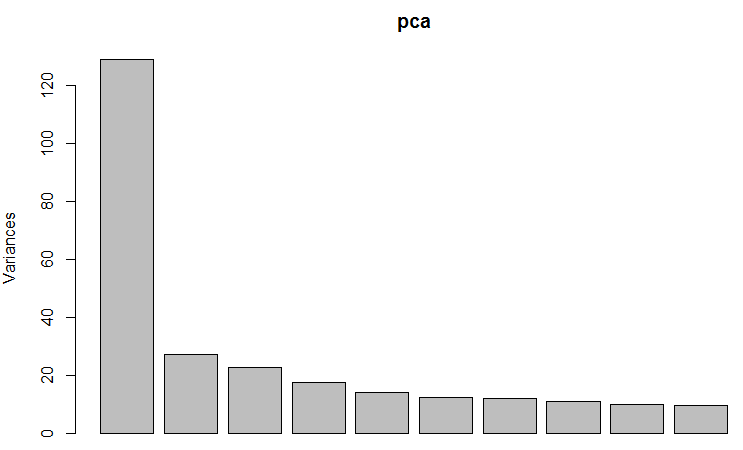
\includegraphics[scale=0.7]{../PCA.PNG}	
	\end{center}
	Therefore, our results are still inconclusive. However, our training Mean Absolute Error was as low as 0.07 for AR(3)MA(1) [takes 3 hours+ to compute]. This is equivalent to 10-20\% erorr rate. [couldn't obtain exact values from the forecast because of small values driving the approximation to infinity and messing up the package's MAPE estimate].
	Our testing however was characterized by overconfidence (really low Standard Error) and volatility (values are really high and fast-changing). This indicates a problem with our ARIMA model that could be rooted in either remaining multicollinearity or simply over-fitting.


	\subsection{Linear Models}:
	The linear model's fit is determined by the in-sample R-squared initially and the Mean Absolute Error for the out-of-sample.
	We estimated the model using the 4 most import lags: 1, 2, 14, 20 and 21. We ignored the MA term in this case.
	The results were an R-squared of 0.98 but when adjusted to the dimensions is more like 0.56 which is still a good correlation value. P-value < 0.01 demonstrates the statistical significance of our variables.
	However, for ease of prediction (1-step ahead prediction for each window) we limited ourselves to the highly autocorrelated 1-lag ($x_{t-1}$). Using lags as far away as 14 and 21 would require a recursive estimation. This is why we are trying to make ARIMA work: once the orders are defined forecasting is trivial. However, for this week, we only did 2 lags + news data.
	Finally, we obtained an MAE of 0.7 which is about 10 times higher than the best in-sample MAE of ARIMA. However, the results made more sense than ARIMA's and as we can see in the graph, they identified major fluctuations in the data with resembling amplitudes. Therefore, the high MAE is rather misleading.
	
	Finally, right before the presentation, we realized a silly error with the preprocessing of the financial time series which might explain the inaccuracies of the ARIMA (why it would overfit this bad) and improve the prediction accuracy of both LM and ARIMA.

\begin{center}
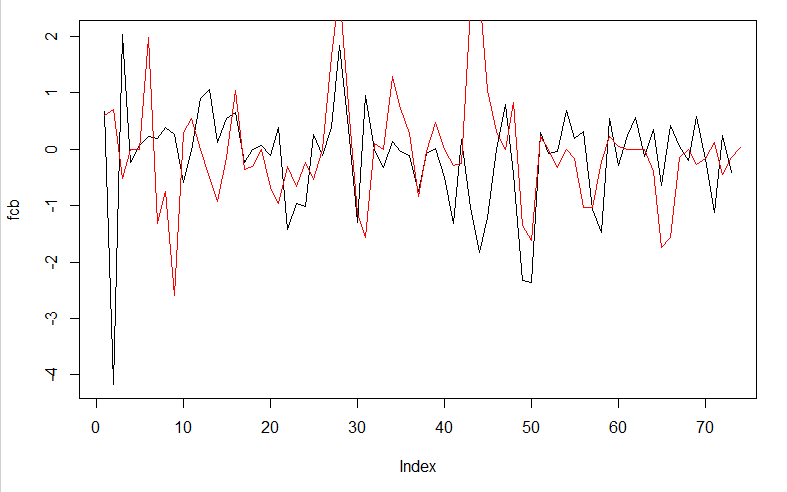
\includegraphics[scale=0.7]{../Pred820.PNG}
\end{center}

	%Tom
	\section{Grid Search for the Most Promising Parameters}
	
        See \hyperref[http://tiny.cc/grid_search_results]{{\color{blue} \underline{grid results online}}}.


	%Vlad
	\section{Kelly trading strategy}
	
The primary means through which our analysis is replicable, falsifiable, and quantitatively assessable is by assessing investment performance. Raw accuracy of prediction does not present a fair evaluation of our algorithm, since we need to consider inherent difficulties with predicting the market. In other words, if we make a significant amount of money (e.g. compare the mean returns to S\&P alpha), then there is some inefficiency in the market that our algorithm correctly enables us to take advantage of.

We will use strong simplifying assumptions: we can trade stock at any volume at the EOD price instantaneously without affecting the market. To some extent these assumptions can hold assuming we create a portfolio of commodities, which artificially lowers market presence in individual ones.

That said, we need to convert our model into an actual strategy. Consider the random variable for the EOD price of a commodity $p_i$ for day $i$. Our LM and ARIMA Models provide for $X = \log\frac{p_{i+1}-p_i}{p_i}$ and $X'=X|p_{<i},\text{news}$ an estimate $\mu=\mathbb{E}(X')$ and $\sigma^2=\mathbb{V}(X')$.

The Kelly Criterion (in the continuous case) gives the optimal betting proportion (given an investment, you should only bet a part of it if you're unsure and leverage it if you aren't). This doesn't make any stronger assumptions about the returns (which should be normal about our prediction) than the models do. Then, each day, we need to buy or short sell $\text{sgn }\mu\cdot\frac{\left|\mu\right|-r}{\sigma^2}$ proportion of our investment, where we sell or buy back all our holdings the next day. We purchase leverage at the risk-free rate $r$, so we only invest when we can earn over that much.

Source: http://wwwf.imperial.ac.uk/~mdavis/docs/DavisLleoKellyChapter.pdf

Here's an example run. The purple line is a trading strategy with $\mu\sim\text{Unif}(-5,5)$ and the tan line has $\mu\sim\text{Unif}(-1,1)$. Both have $\sigma^2\sim\text{Unif}(0.25,10)$. The following has $r=0$:

\begin{center}
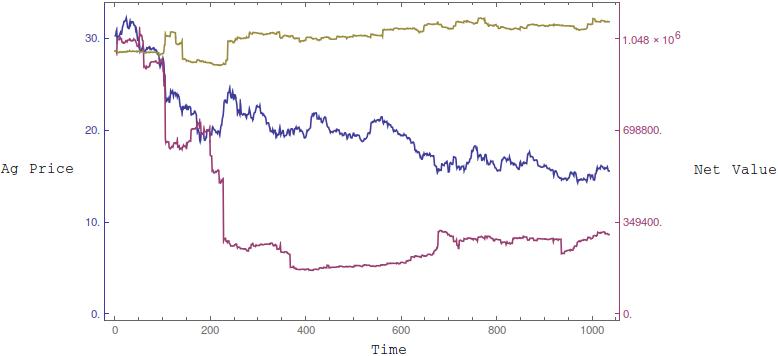
\includegraphics[scale=0.5]{../KellyRun-Random.png}
\end{center}

Notice when we're really confident we tend to leverage {\em a lot}. We might want to have a minimum uncertainty bound, maybe based on stock volatility.

	%Daway
		\section{Clustering}
	
	We attempted using a Dirichlet Process GMM because we have relatively information for deciding how many news clusters there should be. Unfortunately, implementations we attempted to use were intractable given the memory and computing constraints of the ionic cluster. Thus we had to revert back to a $K$-means clustering model.

	We train these models on a set of randomly sampled events for a given date range, for example, the date range of 01-01-2006 to 12-31-2013. Currently we sample 600,000 events across 150 randomly chosen files in this range, weighting the number of events from each day according to the total number of events in that day. Since trading strategies occur day by day, we can train this clustering offline and then make an "online" prediction for which cluster the next day's news data will belong in.

	Since we must do a parameter search across various values for $K$, we do a manual eyeball test to see if clusters make sense. With so many events, values for $K=1000$ or greater seem reasonable. We will present qualitative assessments for some clusters in the $K=1000$ model. It will be easiest to describe the raw news events with the url associated with them.

	Sometimes we can see logical reasons for clusters even if they might not be the most natural or related clusters. For example, cluster 2 has many news related to police:
	\begin{enumerate}
	\item http://www.stgeorgeutah.com/news/archive/2014/12/31/cmm-department-honors-retiring-fire-chief-with-36-booms-and-a-bell/
	\item https://news.vice.com/article/georgia-police-chief-claims-he-accidentally-shot-wife-on-new-years-day
	\item
	http://news.gnom.es/news/nyc-to-ring-in-new-year-with-heightened-security-in-times-square
	\end{enumerate}

	Many times, clusters seem to have many mini-clusters in them. We see this in cluster 345, which has a lot of news related to Israel/Palestine, but also a lot of news related to generate gun violence.
	\begin{enumerate}
	\item http://www.israelherald.com/index.php/sid/228975387
	\item http://www.breakingisraelnews.com/26803/indiana-governor-mike-pence-pledges-support-from-heartland-of-israel-jerusalem/
	\item http://www.thedenverchannel.com/newsy/how-palestinian-leaders-latest-move-could-backfire
	\item http://www.erietvnews.com/story/27744858/mahmoud-abbas-fast-facts
	\item http://www.bostonglobe.com/metro/2015/01/01/brandeis-student-stands-comments-after-slayings-new-york-police-officers/oLpI7MiV42hk3ymM05QzLN/story.html
	\item http://www.toledoblade.com/State/2015/01/01/Cleveland-seeks-outside-probe-of-boy-s-shooting.html
	\end{enumerate}

	There were many clusters that had good topic clustering, such as general politics clusters, which would contain news about gubernatorial elections, general actions by President Obama, and some foreign policy news. But overall, these clusters were disappointing since they didn't leverage geographic location to separate clusters that way which we would have suspected. 

	One of the best clusters found had to do with general crime and legal issues, though again, geographic information does not seem to have affected clustering much. We also note that the magnitude or importance of these events does not seem to match up.
	\begin{enumerate}
	\item http://blogs.reuters.com/faithworld/2015/01/01/new-zealand-bar-manager-pleads-not-guilty-to-insulting-buddhism-in-myanmar/
	\item http://www.hstoday.us/blogs/the-kimery-report/blog/cia-might-have-avoided-post-911-torture-charges-had-it-remembered-beirut-1983/eb540ef9ce52b4a80f490369e743e4fb.html
	\item http://www.military.com/daily-news/2015/01/01/us-sends-5-detainees-to-kazakhstan-a-day-late.html?comp=700001075741rank=4
	\item http://aninews.in/newsdetail4/story197991/lakhvi-sent-to-14-days-judicial-custody-in-kidnapping-case.html
	\item http://www.sasklifestyles.com/news/police-say-mother-of-missing-14-month-old-maryland-boy-left-him-on-stranger-s-porch-in-ohio-1.1700200
	\end{enumerate}

	Overall, most clusters had some sort of relating factor for its news events. But the main problems we can identify are the existence of multiple mini clusters and the division of true clusters across many clusters. The second point might be less worrisome, since the $K$-means algorithm may have split these "true clusters" because of magnitude and importance features which are harder to eyeball than assigning topics.
\begin{enumerate}
\item http://blogs.reuters.com/faithworld/2015/01/01/new-zealand-bar-manager-pleads-not-guilty-to-insulting-buddhism-in-myanmar/
\item http://www.hstoday.us/blogs/the-kimery-report/blog/cia-might-have-avoided-post-911-torture-charges-had-it-remembered-beirut-1983/eb540ef9ce52b4a80f490369e743e4fb.html
\item http://www.military.com/daily-news/2015/01/01/us-sends-5-detainees-to-kazakhstan-a-day-late.html?comp=700001075741rank=4
\item http://aninews.in/newsdetail4/story197991/lakhvi-sent-to-14-days-judicial-custody-in-kidnapping-case.html
\item http://www.sasklifestyles.com/news/police-say-mother-of-missing-14-month-old-maryland-boy-left-him-on-stranger-s-porch-in-ohio-1.1700200
\end{enumerate}

Overall, most clusters had some sort of relating factor for its news events. But the main problems we can identify are the existance of multiple mini clusters and the division of true clusters across many clusters. The second point might be less worrisome, since the $K$-means algorithm may have split these "true clusters" because of magnitude and importance features which are harder to eyeball than assigning topics. 

\end{document}
